\documentclass[10pt,a4paper]{article}
\usepackage[utf8]{inputenc}
\usepackage[a4paper, margin=1.25cm, top=1.30cm, bottom=1.30cm]{geometry}
\usepackage{amsmath,amssymb}
\usepackage{xcolor}
\usepackage[most]{tcolorbox}
\usepackage{booktabs}
\usepackage{colortbl}
\usepackage{fancyhdr}
\usepackage{graphicx}
\usepackage{enumitem}
\usepackage{needspace}
\usepackage{array}

% Exact colors from previous lecture notes
\definecolor{themeblue}{rgb}{0.1686, 0.3529, 0.5294}   % #2B5A87
\definecolor{lightbg}{rgb}{0.9098, 0.9333, 0.9569}     % #E8EEF4
\definecolor{accentred}{rgb}{0.7843, 0.2706, 0.2275}   % #C8453A
\definecolor{accentgreen}{rgb}{0.1804, 0.4902, 0.1961} % #2E7D32
\definecolor{codebg}{rgb}{0.96, 0.97, 0.98}

% Header and Footer
\pagestyle{fancy}
\fancyhf{}
\fancyhead[L]{\textcolor{themeblue}{\small Lecture 6 --- Introduction to Neural Networks (NN 1)}}
\fancyhead[R]{\textcolor{themeblue}{\small Deep Learning}}
\renewcommand{\headrulewidth}{0.5pt}
\renewcommand{\headrule}{\hbox to\headwidth{\color{themeblue}\leaders\hrule height \headrulewidth\hfill}}
\fancyfoot[C]{\thepage}

\begin{document}

% =========================================================================
% PAGE 1: Architecture, Notations, Dimensional Shapes & Matrix Ordering
% =========================================================================

% Title Block
\begin{center}
    {\LARGE\bfseries\color{themeblue} Neural Networks: Architecture, Optimization \& Regularization}\\[1.5pt]
    {\small\itshape Deep Learning (S.-A. Berrani, ENSIA 2026--2027)}\\[1.5pt]
    \textcolor{themeblue}{\rule{\textwidth}{0.5pt}}
\end{center}

\vspace{-12pt}

% Overview Box
\begin{tcolorbox}[
    colframe=themeblue,
    colback=lightbg,
    coltitle=white,
    fonttitle=\bfseries\sffamily\small,
    title={Lecture Scope \& Key Themes},
    arc=1.3mm,
    boxrule=0.5pt,
    left=5pt, right=5pt, top=2pt, bottom=2pt
]
\footnotesize
\textbf{Core Concepts:} Transition from single-neuron logistic regression to multilayer \textbf{Deep Feedforward Neural Networks (DNN)}.
\begin{itemize}[leftmargin=10pt, itemsep=0pt, topsep=0pt]
    \item \textbf{Architectural Representation:} Layer indexing ($l \in \{0, \dots, L\}$), activation vectors $a^{[l]}$, weight matrices $W^{[l]}$, and bias vectors $b^{[l]}$.
    \item \textbf{Non-Linearity:} Roles of activation functions ($\sigma, \tanh, \text{ReLU}, \text{Leaky ReLU}$) and mathematical proof of why linear activations fail.
    \item \textbf{Practical Optimization:} Train/Dev/Test data splitting, Cross-Validation, and input feature normalization.
    \item \textbf{Generalization Mastery:} Bias vs. Variance diagnosis, Bayes error baselines, and $L_1$ vs. $L_2$ regularization mechanisms.
\end{itemize}
\end{tcolorbox}

\vspace{-4pt}

% Section 1: Architecture and Notation
\noindent{\large\bfseries\color{themeblue} 1. Feedforward Neural Network Convention \& Matrix Representation}\par\vspace{1pt}
A general $L$-layer feedforward neural network maps an input feature vector $x \in \mathbb{R}^{n_x}$ through $L-1$ hidden layers to produce prediction $\hat{y} = a^{[L]}$.

\begin{center}
\vspace{-4pt}
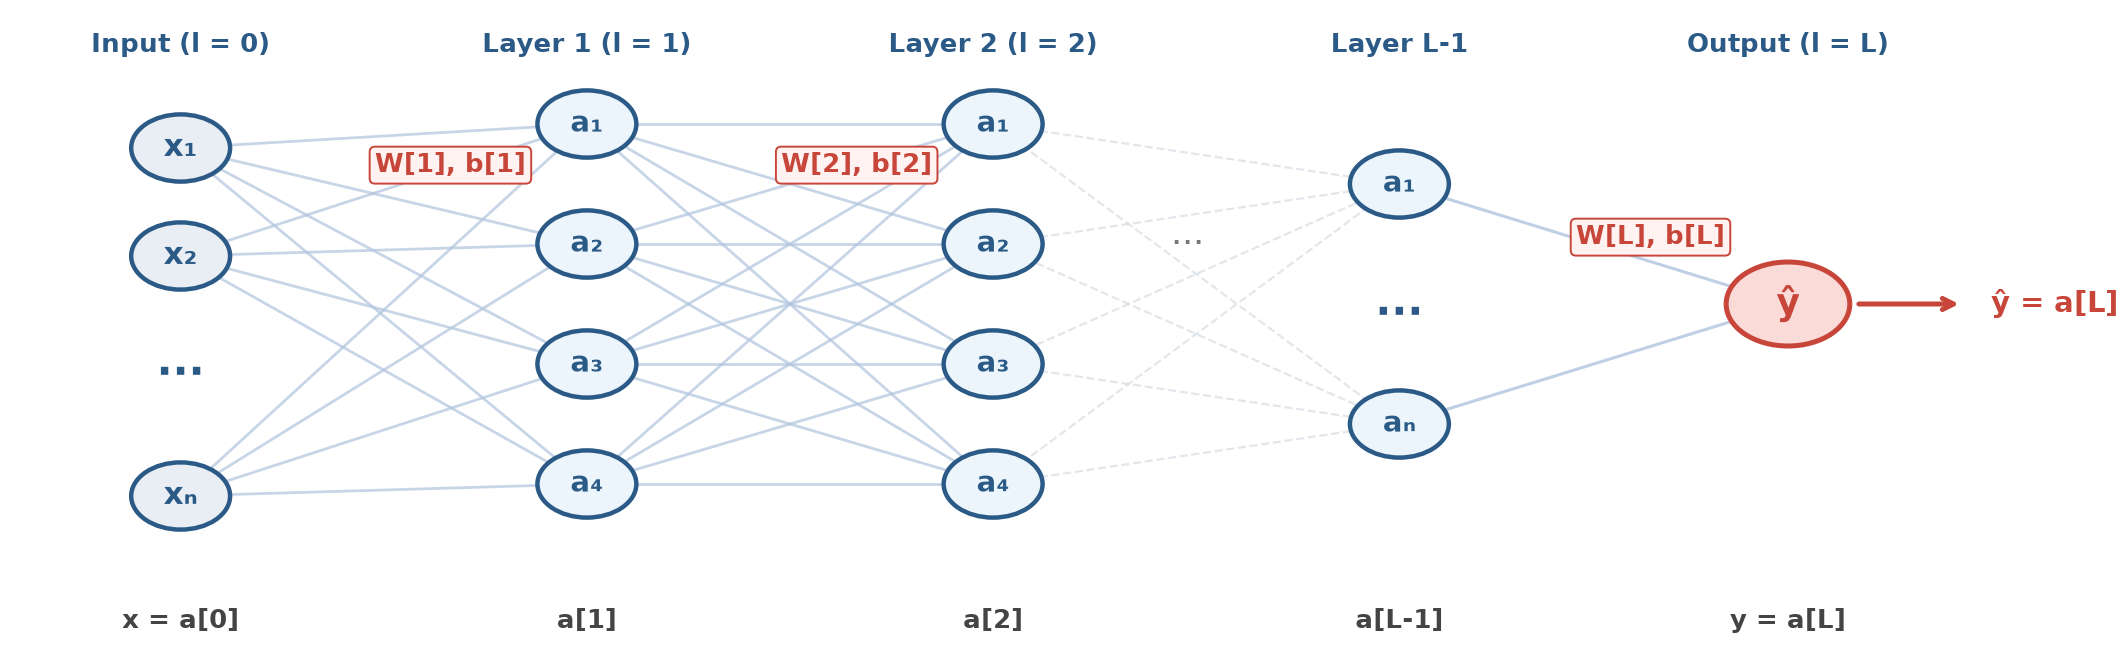
\includegraphics[width=0.68\textwidth]{nn1_architecture.png}\\[-1pt]
{\footnotesize\textit{General $L$-layer Feedforward Neural Network architecture: Inputs $x = a^{[0]}$, intermediate activations $a^{[l]}$, parameters $W^{[l]}, b^{[l]}$, and output $\hat{y} = a^{[L]}$.}}
\end{center}

\vspace{-6pt}

\begin{itemize}[leftmargin=10pt, itemsep=1pt, topsep=0.5pt]
    \item \textbf{Layer Indexing:} Layer $0$ denotes the input layer. Layers $1$ through $L-1$ are \textbf{hidden layers}. Layer $L$ is the \textbf{output layer}.
    \item \textbf{Dimensional Shapes (Single Training Instance):}
    \begin{itemize}[leftmargin=8pt, itemsep=0.5pt]
        \item Input vector: $x = a^{[0]} \in \mathbb{R}^{n^{[0]}}$ where $n^{[0]} = n_x$ features ($x = [x_1, x_2, \dots, x_n]^T$).
        \item Layer $l$ has $n^{[l]}$ neurons: Linear logit $z^{[l]} \in \mathbb{R}^{n^{[l]} \times 1}$, Activation vector $a^{[l]} = g^{[l]}(z^{[l]}) \in \mathbb{R}^{n^{[l]} \times 1}$.
        \item Weight matrix: $W^{[l]} \in \mathbb{R}^{n^{[l]} \times n^{[l-1]}}$, Bias vector: $b^{[l]} \in \mathbb{R}^{n^{[l]} \times 1}$.
    \end{itemize}
    \item \textbf{Vectorized Batch Computation ($m$ Training Examples):}
    Stacking $m$ sample vectors horizontally as columns creates design matrices:
    \begin{align*}
    X = A^{[0]} &= \big[x^{(1)}, x^{(2)}, \dots, x^{(m)}\big] \in \mathbb{R}^{n_x \times m} \\[1pt]
    Z^{[l]} &= W^{[l]} A^{[l-1]} + b^{[l]} \in \mathbb{R}^{n^{[l]} \times m}, \qquad A^{[l]} = g^{[l]}\big(Z^{[l]}\big) \in \mathbb{R}^{n^{[l]} \times m}
    \end{align*}
    where $b^{[l]} \in \mathbb{R}^{n^{[l]} \times 1}$ is automatically broadcasted across all $m$ columns.
\end{itemize}

\vspace{-3pt}

\begin{tcolorbox}[
    colframe=accentred,
    colback=white,
    arc=1.3mm,
    boxrule=0.5pt,
    left=5pt, right=5pt, top=2pt, bottom=2pt
]
\footnotesize
\textbf{Weight Matrix Internal Structure ($W^{[l]} \in \mathbb{R}^{n^{[l]} \times n^{[l-1]}}$):}
\[
W^{[l]} = 
\begin{bmatrix}
\text{---} & (w_1^{[l]})^T & \text{---} \\
\text{---} & (w_2^{[l]})^T & \text{---} \\
& \vdots & \\
\text{---} & (w_{n^{[l]}}^{[l]})^T & \text{---}
\end{bmatrix}
=
\begin{bmatrix}
w_{1, 1}^{[l]} & w_{1, 2}^{[l]} & \cdots & w_{1, n^{[l-1]}}^{[l]} \\
w_{2, 1}^{[l]} & w_{2, 2}^{[l]} & \cdots & w_{2, n^{[l-1]}}^{[l]} \\
\vdots & \vdots & \ddots & \vdots \\
w_{n^{[l]}, 1}^{[l]} & w_{n^{[l]}, 2}^{[l]} & \cdots & w_{n^{[l]}, n^{[l-1]}}^{[l]}
\end{bmatrix}
\]
\begin{itemize}[leftmargin=8pt, itemsep=0.5pt, topsep=0.5pt]
    \item \textbf{Row Vectors (Row $i$ of $W^{[l]}$):} Each row vector $(w_i^{[l]})^T$ contains the weights connecting \textbf{all different incoming inputs} $j \in \{1, \dots, n^{[l-1]}\}$ from layer $l-1$ into that \textbf{same single destination neuron $i$} in layer $l$:
    \[
    z_i^{[l]} = \sum_{j=1}^{n^{[l-1]}} W_{i, j}^{[l]} \, a_j^{[l-1]} + b_i^{[l]} = (w_i^{[l]})^T a^{[l-1]} + b_i^{[l]}
    \]
    \item \textbf{Column Vectors (Column $j$ of $W^{[l]}$):} Each column vector $[W^{[l]}]_{:, j}$ collects the weights fanning out from the \textbf{same incoming input neuron $j$} in layer $l-1$ going to \textbf{all different output neurons} $i \in \{1, \dots, n^{[l]}\}$ in layer $l$.
    \item \textit{Note on Transposed Conventions:} In libraries computing $z^T = a^T W + b^T$, $W$ has shape $n^{[l-1]} \times n^{[l]}$, swapping row/column roles. In standard DL / Andrew Ng convention, $W^{[l]}$ is strictly $(n^{[l]} \times n^{[l-1]})$.
\end{itemize}
\end{tcolorbox}

\newpage

% =========================================================================
% PAGE 2: Activation Functions, Non-Linearity Proof & Hyperparameters
% =========================================================================

\noindent{\large\bfseries\color{themeblue} 2. Activation Functions: Properties, Formulas \& Non-Linearity}\par\vspace{1pt}
Activation functions introduce non-linear transformations into network nodes, granting neural networks universal function approximation capabilities.

\begin{center}
\vspace{-3pt}
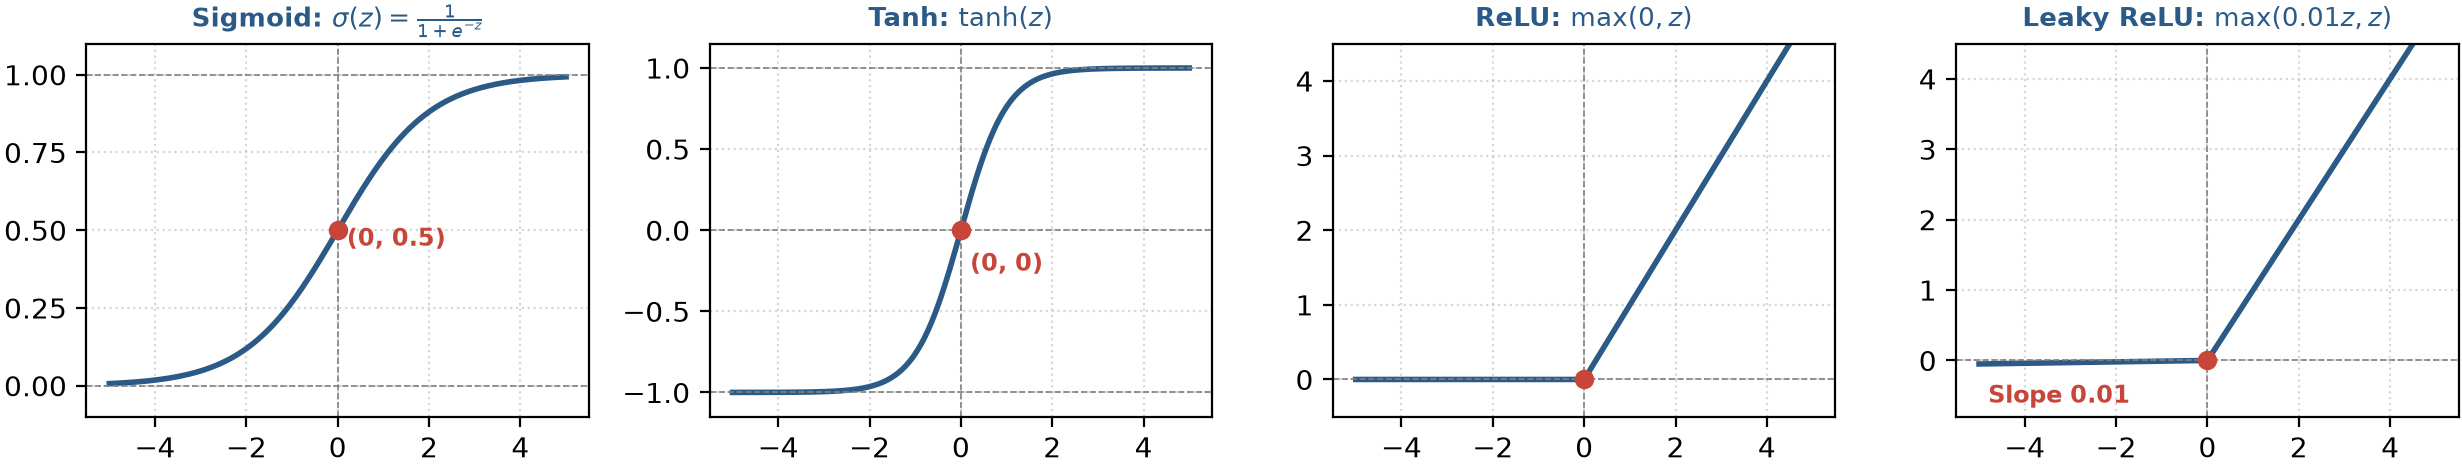
\includegraphics[width=0.88\textwidth]{nn1_activations.png}\\[-1pt]
{\footnotesize\textit{Comparison of primary activation functions: Sigmoid $\sigma(z)$, Hyperbolic Tangent $\tanh(z)$, Rectified Linear Unit ($\text{ReLU}$), and $\text{Leaky ReLU}$.}}
\end{center}

\vspace{-6pt}

\begin{center}
\footnotesize
\setlength{\tabcolsep}{3pt}
\begin{tabular}{>{\raggedright\arraybackslash}p{0.15\textwidth}>{\raggedright\arraybackslash}p{0.22\textwidth}>{\raggedright\arraybackslash}p{0.12\textwidth}>{\raggedright\arraybackslash}p{0.16\textwidth}>{\raggedright\arraybackslash}p{0.29\textwidth}}
\toprule
\rowcolor{lightbg}
\textbf{Activation} & \textbf{Formula $g(z)$} & \textbf{Range} & \textbf{Derivative $g'(z)$} & \textbf{Primary Usage \& Notes} \\
\midrule
\textbf{Sigmoid} & $g(z) = \dfrac{1}{1 + e^{-z}}$ & $(0, 1)$ & $g(z)(1 - g(z))$ & Output layer for binary classification; vanishing gradients for $|z| > 4$. \\
\addlinespace[1.5pt]
\textbf{Tanh} & $g(z) = \dfrac{e^z - e^{-z}}{e^z + e^{-z}}$ & $(-1, 1)$ & $1 - g(z)^2$ & Zero-centered hidden layers ($\mu \approx 0$); saturates for $|z| > 3$. \\
\addlinespace[1.5pt]
\textbf{ReLU} & $g(z) = \max(0, z)$ & $[0, +\infty)$ & $\begin{cases} 1 & z > 0 \\ 0 & z < 0 \end{cases}$ & Standard default for hidden layers; lightning fast, solves vanishing gradients for $z > 0$; "dying ReLU" risk. \\
\addlinespace[1.5pt]
\textbf{Leaky ReLU} & $g(z) = \max(0.01z, z)$ & $(-\infty, +\infty)$ & $\begin{cases} 1 & z > 0 \\ 0.01 & z < 0 \end{cases}$ & Prevents dead neurons by passing a subtle gradient ($0.01$) when $z \le 0$. \\
\bottomrule
\end{tabular}
\end{center}

\vspace{-3pt}

\noindent{\bfseries\color{themeblue} Why Do We Need Non-Linearity?}\par
\begin{itemize}[leftmargin=10pt, itemsep=1pt, topsep=0.5pt]
    \item Real-world problems (computer vision, audio, complex classification) exhibit intricately folded, non-linear decision manifolds.
    \item A linear function has a single, constant slope everywhere. Non-linear functions possess a \textbf{continuously varying slope}, allowing localized feature sensitivity and complex pattern composition.
\end{itemize}

\vspace{-2pt}

% Proof Box: Linear Activation Collapses NN
\begin{tcolorbox}[
    colframe=themeblue,
    colback=lightbg,
    coltitle=white,
    fonttitle=\bfseries\sffamily\small,
    title={Formal Proof: An $L$-Layer Linear Activation Network is Pointless},
    arc=1.3mm,
    boxrule=0.5pt,
    left=5pt, right=5pt, top=2pt, bottom=2pt
]
\footnotesize
\textbf{Theorem:} If all activation functions are linear, i.e., $g^{[l]}(z) = z$ for all $l \in \{1, \dots, L\}$, an arbitrary $L$-layer neural network collapses into a simple linear affine model.
\\[1.5pt]
\textbf{Derivation:}
\begin{align*}
\text{Layer 1:} \quad a^{[1]} &= z^{[1]} = W^{[1]} x + b^{[1]} \\[1pt]
\text{Layer 2:} \quad a^{[2]} &= z^{[2]} = W^{[2]} a^{[1]} + b^{[2]} = W^{[2]} \big(W^{[1]} x + b^{[1]}\big) + b^{[2]} = \underbrace{\big(W^{[2]} W^{[1]}\big)}_{W'} x + \underbrace{\big(W^{[2]} b^{[1]} + b^{[2]}\big)}_{b'} = W' x + b' \\[1pt]
\text{Layer 3:} \quad a^{[3]} &= z^{[3]} = W^{[3]} a^{[2]} + b^{[3]} = W^{[3]}\big(W' x + b'\big) + b^{[3]} = W'' x + b''
\end{align*}
By induction, for an arbitrary depth $L$: $a^{[L]} = \widetilde{W} x + \tilde{b}$ where $\widetilde{W} = \prod_{l=L}^1 W^{[l]} \in \mathbb{R}^{n^{[L]} \times n_x}$.\\[1.5pt]
\textbf{Conclusion:} Composition of linear functions is strictly linear. No matter how many layers or units are stacked, a linear neural network cannot compute anything beyond basic linear regression (or 1-layer logistic regression if final activation is sigmoid). All hidden layers are computationally redundant.
\end{tcolorbox}

\vspace{-2pt}

% Section 3: Parameters vs Hyperparameters
\noindent{\large\bfseries\color{themeblue} 3. Model Parameters vs. Hyperparameters}\par\vspace{1pt}
\begin{itemize}[leftmargin=10pt, itemsep=1pt, topsep=0.5pt]
    \item \textbf{Trainable Parameters:} Internal variables optimized by gradient descent:
    $\{W^{[1]}, b^{[1]}, W^{[2]}, b^{[2]}, \dots, W^{[L]}, b^{[L]}\}$.
    \item \textbf{Hyperparameters:} External controls set by the practitioner:
    Learning rate $\alpha$, number of layers $L$, neurons per layer $n^{[l]}$, iterations/epochs, activation functions $g^{[l]}$, regularization parameter $\lambda$, mini-batch size.
    \item \textbf{The Iterative Empirical Process:}
    \[
    \boxed{\text{\bfseries Idea}} \;\longrightarrow\; \boxed{\text{\bfseries Code / Architecture}} \;\longrightarrow\; \boxed{\text{\bfseries Experiment}} \;\longrightarrow\; \boxed{\text{\bfseries Tune Hyperparameters}}
    \]
\end{itemize}

\newpage

% =========================================================================
% PAGE 3: Data Splitting, Cross-Validation & Normalization
% =========================================================================

\noindent{\large\bfseries\color{themeblue} 4. Dataset Splitting Strategy \& Cross-Validation}\par\vspace{1pt}
To rigorously train and evaluate deep neural networks, available data is split into three disjoint subsets:
\begin{enumerate}[leftmargin=12pt, itemsep=1pt, topsep=0.5pt]
    \item \textbf{Training Set:} Used directly by backpropagation to fit model parameters $(W^{[l]}, b^{[l]})$.
    \item \textbf{Development (Dev / Validation) Set:} Used to evaluate candidate architectures, tune hyperparameters ($\alpha, \lambda, n^{[l]}$), and diagnose bias/variance.
    \item \textbf{Test Set:} Evaluated \textbf{only once} at the very end to provide an unbiased estimate of real-world generalization error.
\end{enumerate}

\vspace{-2pt}

\begin{tcolorbox}[
    colframe=themeblue, colback=lightbg, arc=1.3mm, boxrule=0.5pt,
    left=5pt, right=5pt, top=2pt, bottom=2pt
]
\footnotesize
\textbf{Maximizing the Training Set in Modern Deep Learning:}
\begin{itemize}[leftmargin=8pt, itemsep=1pt, topsep=0pt]
    \item \textbf{Traditional ML Era ($m \le 10{,}000$):} Data was scarce. Common splits were $70\% / 30\%$ (Train/Test) or $60\% / 20\% / 20\%$ (Train/Dev/Test).
    \item \textbf{Big Data \& Deep Learning Era ($m \ge 1{,}000{,}000$):} Deep networks are heavily parameterized and \textbf{data-hungry}. Therefore, we always seek to \textbf{maximize the training set}.
    \item \textbf{Sufficiency Rationale:} The Dev and Test sets only require enough absolute samples to provide statistical significance (e.g., $10{,}000$ samples suffice to confidently distinguish a $1.1\%$ error from a $1.2\%$ error).
    \item \textbf{Example:} With $m = 1{,}000{,}000$ examples:
    \[
    \mathbf{98\% \text{ Train}} \ (980\text{k}) \quad\Big|\quad \mathbf{1\% \text{ Dev}} \ (10\text{k}) \quad\Big|\quad \mathbf{1\% \text{ Test}} \ (10\text{k})
    \]
    \item \textbf{Identical Distribution Rule:} Train, Dev, and Test sets \textbf{must come from the exact same probability distribution}. Mismatched distributions invalidate validation diagnostics.
\end{itemize}
\end{tcolorbox}

\vspace{-3pt}

\noindent{\bfseries\color{themeblue} Cross-Validation Procedure:}\par
When total dataset size is small ($m < 10{,}000$), holding out a dedicated dev set sacrifices valuable training data. We apply \textbf{$k$-fold Cross-Validation}: partition data into $k$ equal folds, iteratively train on $k-1$ folds and validate on the remaining fold, then average validation performance across all $k$ rounds. In large-scale deep learning ($m \ge 10^5$), standard single Dev/Test splits are preferred due to computational cost.

\vspace{1pt}

% Section 5: Normalization
\noindent{\large\bfseries\color{themeblue} 5. Normalization of Input Feature Vectors}\par\vspace{1pt}
Feature normalization transforms raw inputs into a zero-centered, unit-variance space:

\begin{center}
\vspace{-4pt}
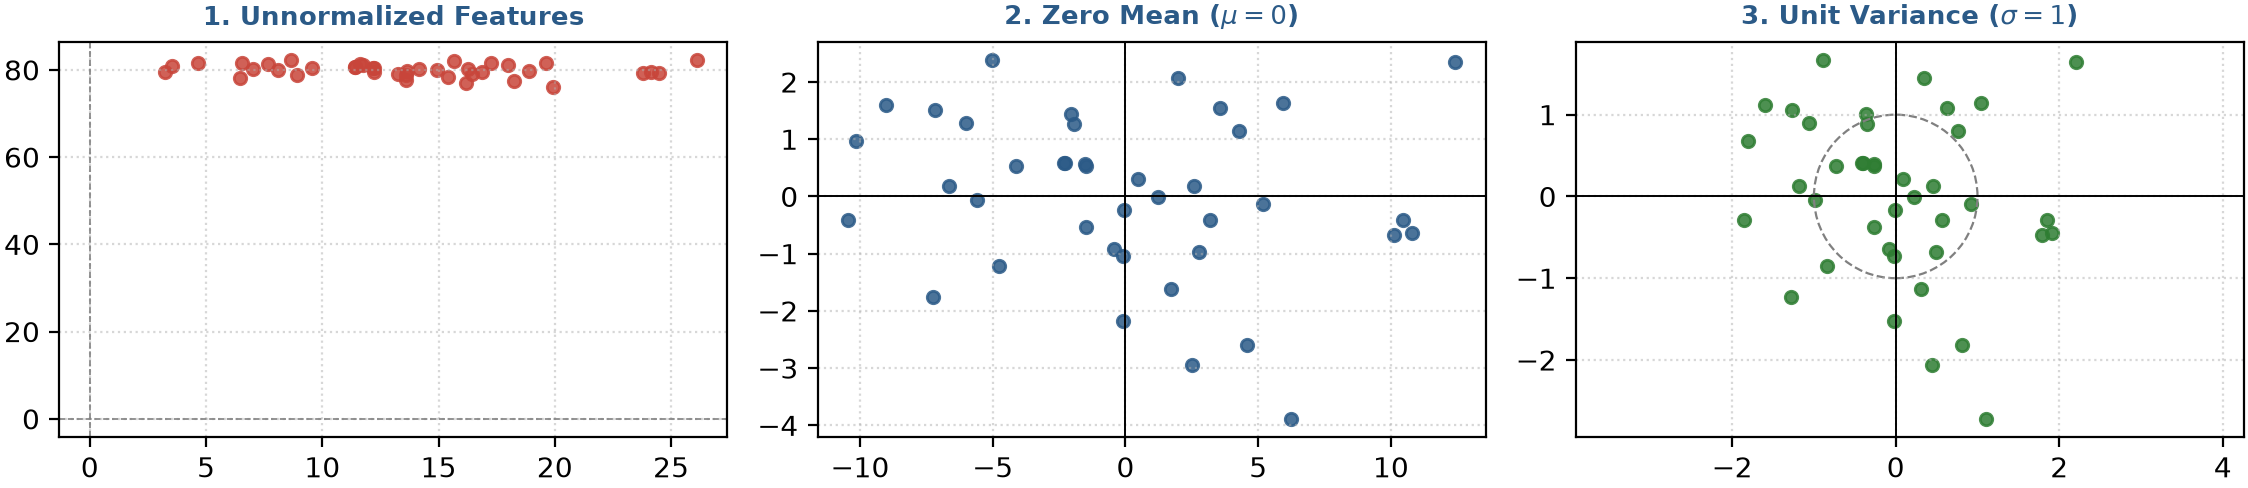
\includegraphics[width=0.82\textwidth]{nn1_normalization.png}\\[-1pt]
{\footnotesize\textit{Two-step normalization process: (1) Raw unnormalized features $\to$ (2) Zero-mean centering $\to$ (3) Variance normalization.}}
\end{center}

\vspace{-6pt}

\begin{enumerate}[leftmargin=12pt, itemsep=1.5pt, topsep=0.5pt]
    \item \textbf{Step 1: Zero-Mean Centering:} Compute empirical mean $\mu \in \mathbb{R}^{n_x}$ and subtract:
    \[
    \mu = \frac{1}{m} \sum_{i=1}^m x^{(i)}, \qquad x := x - \mu
    \]
    \item \textbf{Step 2: Variance Normalization:} Compute coordinate-wise variance $\sigma^2 \in \mathbb{R}^{n_x}$ and scale:
    \[
    \sigma^2 = \frac{1}{m} \sum_{i=1}^m \big(x^{(i)}\big)^2, \qquad x := \frac{x}{\sigma} \qquad (\sigma = \sqrt{\sigma^2 + \epsilon})
    \]
\end{enumerate}

\begin{center}
\vspace{-4pt}
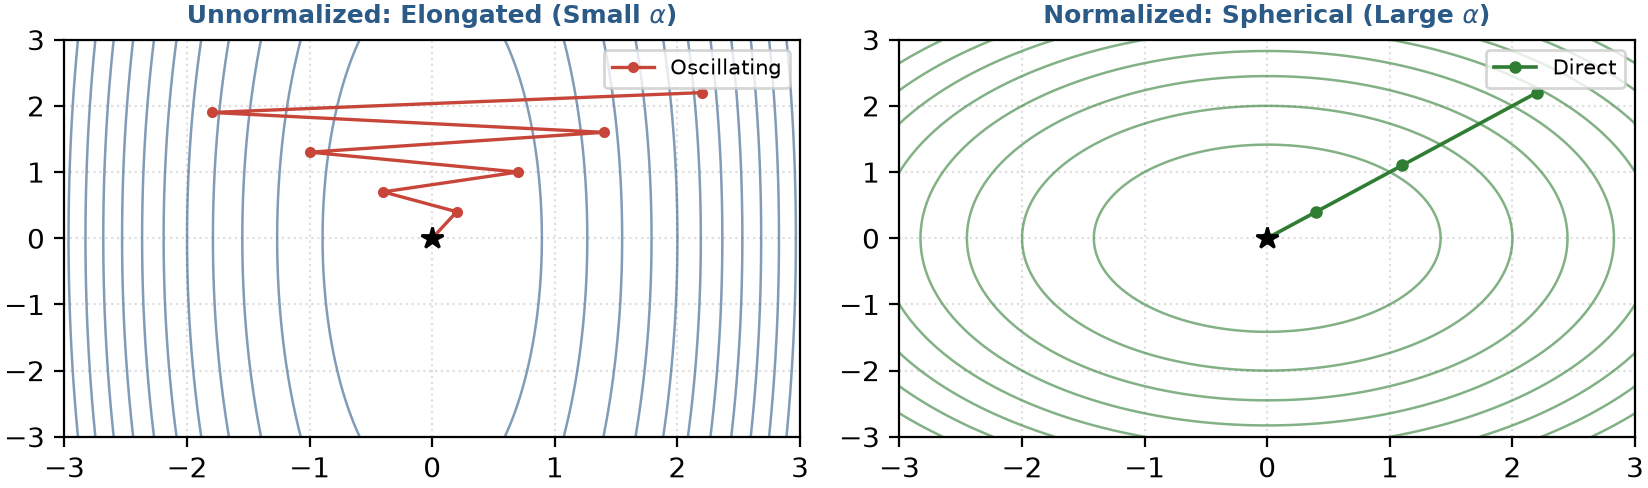
\includegraphics[width=0.62\textwidth]{nn1_contours.png}\\[-1pt]
{\footnotesize\textit{Cost function contours: Elongated bowl forces oscillating zig-zag paths vs. Spherical contours enabling direct, rapid descent.}}
\end{center}

\vspace{-6pt}

\begin{tcolorbox}[
    colframe=accentred, colback=white, arc=1.3mm, boxrule=0.5pt,
    left=5pt, right=5pt, top=2pt, bottom=2pt
]
\footnotesize
\textbf{Why Do We Normalize? Geometric \& Numerical Explanation:}
\begin{itemize}[leftmargin=8pt, itemsep=0.5pt, topsep=0pt]
    \item If features have wildly different ranges (e.g., $x_1 \in [0, 1]$ and $x_2 \in [1000, 100000]$), weights $w_1, w_2$ exhibit vastly different gradient scales. The loss function surface becomes an \textbf{elongated, highly eccentric elliptical valley} (ill-conditioned Hessian matrix).
    \item In unnormalized terrain, gradient descent oscillates violently perpendicular to the valley, forcing an agonizingly small learning rate $\alpha$ to prevent divergence.
    \item After normalization, loss contours are \textbf{spherical (isotropic)}. Gradients point directly toward the global minimum, allowing a much larger learning rate $\alpha$ and drastically accelerating convergence.
    \item \textbf{CRITICAL RULE:} Normalization parameters $(\mu, \sigma)$ calculated on the \textbf{Train set} must be reused without recomputation on Dev and Test sets to prevent data leakage.
\end{itemize}
\end{tcolorbox}

\newpage

% =========================================================================
% PAGE 4: Bias & Variance Diagnosis and Flowchart
% =========================================================================

\noindent{\large\bfseries\color{themeblue} 6. Bias and Variance: Mathematical Formulation \& Diagnostics}\par\vspace{1pt}
Evaluating the generalization capabilities of a trained model requires examining the gap between training and validation error.

\begin{tcolorbox}[
    colframe=themeblue, colback=lightbg, coltitle=white,
    fonttitle=\bfseries\sffamily\small,
    title={Mathematical Definition: Bias-Variance Decomposition},
    arc=1.3mm, boxrule=0.5pt, left=5pt, right=5pt, top=2pt, bottom=2pt
]
\footnotesize
For an estimation task with target $y = f(x) + \epsilon$ where $\mathbb{E}[\epsilon] = 0, \text{Var}(\epsilon) = \sigma_\epsilon^2$, expected test error decomposes cleanly:
\[
\mathbb{E}_{\mathcal{D}}\big[(y - \hat{f}(x))^2\big] = \underbrace{\Big(\mathbb{E}_{\mathcal{D}}[\hat{f}(x)] - f(x)\Big)^2}_{\textbf{Bias}^2} + \underbrace{\mathbb{E}_{\mathcal{D}}\Big[\big(\hat{f}(x) - \mathbb{E}_{\mathcal{D}}[\hat{f}(x)]\big)^2\Big]}_{\textbf{Variance}} + \underbrace{\sigma_\epsilon^2}_{\textbf{Irreducible Error}}
\]
\begin{itemize}[leftmargin=8pt, itemsep=0.5pt, topsep=0pt]
    \item \textbf{Bias:} $\text{Bias}[\hat{f}(x)] = \mathbb{E}[\hat{f}(x)] - f(x)$. Measures how much the \textbf{average of all predictions} across different partitions / training subsets of the data differs from the \textbf{actual ground truth} $f(x)$ due to overly simplistic model assumptions ($\implies$ \textbf{Underfitting}).
    \item \textbf{Variance:} $\text{Var}[\hat{f}(x)] = \mathbb{E}\big[(\hat{f}(x) - \mathbb{E}[\hat{f}(x)])^2\big]$. Measures the \textbf{variance (dispersion)} between all the different individual predictions across different data partitions around their mean, capturing sensitivity to sample noise ($\implies$ \textbf{Overfitting}).
    \item \textbf{Irreducible Error ($\sigma_\epsilon^2$):} Inherent noise in the data generating process (Bayes optimal error).
\end{itemize}
\end{tcolorbox}

\vspace{-3pt}

\noindent{\bfseries\color{themeblue} Diagnosing Bias vs. Variance: Benchmark Comparison:}\par
Diagnosis relies on comparing \textbf{Train Set Error} vs. \textbf{Dev Set Error} relative to the \textbf{Human-Level (Bayes Optimal) Error}:

\vspace{1pt}
\begin{center}
\footnotesize
\setlength{\tabcolsep}{3pt}
\begin{tabular}{p{0.26\textwidth}p{0.16\textwidth}p{0.16\textwidth}p{0.20\textwidth}p{0.16\textwidth}}
\toprule
\rowcolor{lightbg}
\textbf{Metric / Benchmark} & \textbf{Case A} & \textbf{Case B} & \textbf{Case C} & \textbf{Case D} \\
\midrule
\textbf{Train Error} & $0.5\%$ & $18\%$ & $18\%$ & $2\%$ \\
\textbf{Dev Error} & $10\%$ & $19\%$ & $35\%$ & $3\%$ \\
\midrule
\textbf{Human Error = 0\%:} & \textbf{High Variance} & \textbf{High Bias} & \textbf{High Bias \& High Var} & \textbf{Low Bias \& Low Var} \\
\midrule
\textbf{Human Error = 16\%:} & \textbf{High Variance} & \textbf{Low Bias \& Low Var} & \textbf{High Bias} ($30\%$ vs $32\%$) & \textbf{Low Bias \& Low Var} \\
\bottomrule
\end{tabular}
\end{center}

\vspace{-3pt}
\begin{itemize}[leftmargin=10pt, itemsep=0.5pt]
    \item \textbf{Avoidable Bias:} Difference between Human-level error (Bayes baseline) and Train error.
    \item \textbf{Variance (Generalization Gap):} Difference between Train error and Dev error.
\end{itemize}

\vspace{-2pt}

\noindent{\bfseries\color{themeblue} Systematic Methodology: What To Do in Case of High Bias or High Variance:}\par

\begin{center}
\vspace{-4pt}
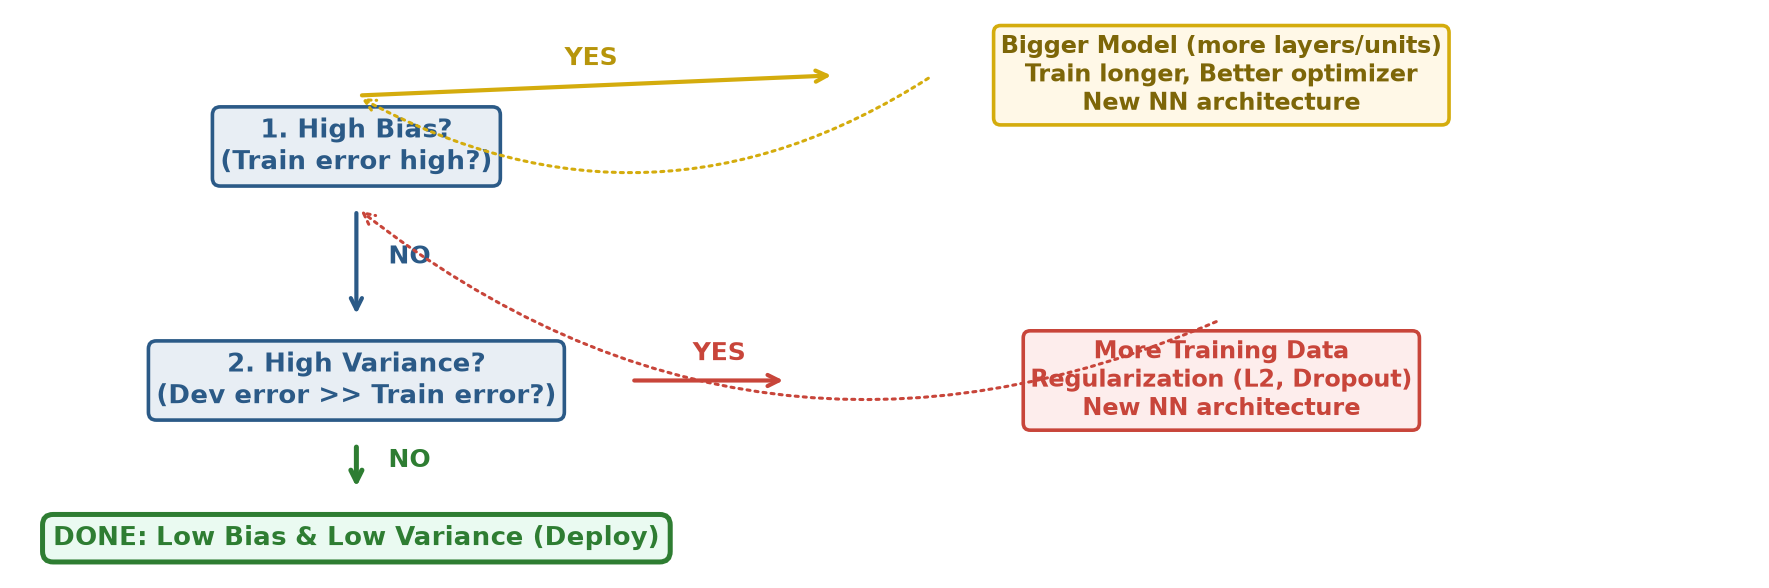
\includegraphics[width=0.72\textwidth]{nn1_flowchart.png}\\[-1pt]
{\footnotesize\textit{Systematic Deep Learning diagnostic workflow: Iterative resolution of bias first, then variance.}}
\end{center}

\vspace{-6pt}

\begin{enumerate}[leftmargin=12pt, itemsep=1pt, topsep=0.5pt]
    \item \textbf{Step 1: Check High Bias (Train set performance):}
    \begin{itemize}[leftmargin=8pt, itemsep=0.5pt]
        \item \textit{Remedies:} Train a bigger model (more layers, more hidden units), train longer, adopt better optimization algorithms (Adam, RMSProp), or search for improved network architectures.
        \item \textit{Loop:} Repeat until training error is close to the human-level / Bayes baseline.
    \end{itemize}
    \item \textbf{Step 2: Check High Variance (Dev set performance):}
    \begin{itemize}[leftmargin=8pt, itemsep=0.5pt]
        \item \textit{Remedies:} Collect more training data, apply \textbf{Regularization} ($L_2$, Dropout, data augmentation), or adjust model architecture.
        \item \textit{Loop:} Repeat until dev set error approaches training error.
    \end{itemize}
    \item \textbf{The Modern Deep Learning Superpower:} In classic ML, reducing bias almost always increased variance (the strict bias-variance tradeoff). In Deep Learning, training a bigger network reduces bias \textbf{without hurting variance}, while collecting data or adding regularization reduces variance \textbf{without hurting bias}!
\end{enumerate}

\newpage

% =========================================================================
% PAGE 5: Regularization (L1 vs L2) & Side-by-Side Mathematical Development
% =========================================================================

\noindent{\large\bfseries\color{themeblue} 7. Regularization: Solutions to Avoid Overfitting ($L_1$ vs. $L_2$)}\par\vspace{1pt}
\textbf{Definition:} Regularization is the process of penalizing model complexity to prevent overfitting and ensure high generalization capacity on unseen data.

\begin{center}
\vspace{-4pt}
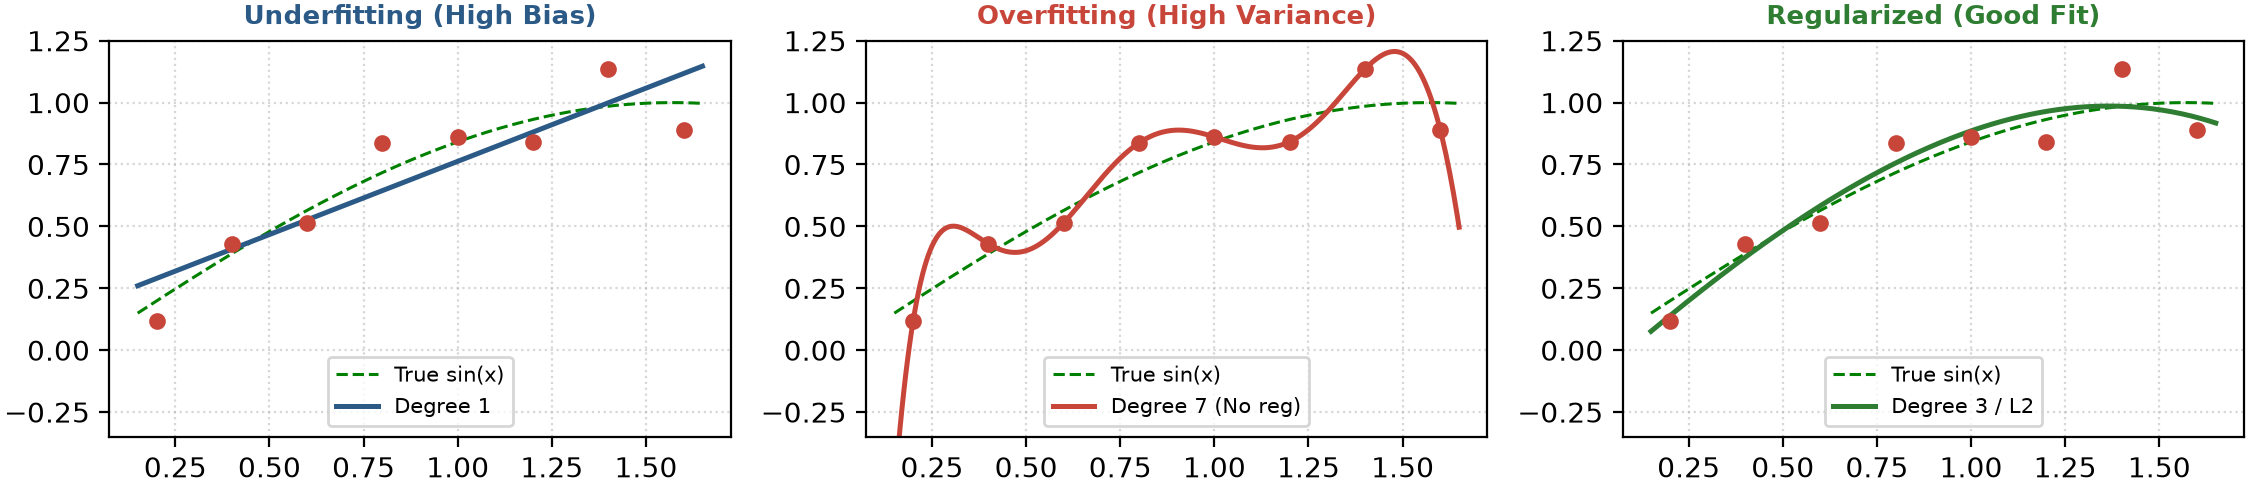
\includegraphics[width=0.82\textwidth]{nn1_poly_fit.png}\\[-1pt]
{\footnotesize\textit{Polynomial fitting comparison: Unregularized high-degree models oscillate violently with massive parameter weights, whereas regularization restricts weight magnitudes to recover the smooth ground truth.}}
\end{center}

\vspace{-6pt}

\begin{itemize}[leftmargin=10pt, itemsep=1pt, topsep=0.5pt]
    \item \textbf{Optimization Objective:}
    $\min_{w, b} \mathcal{J}(w, b) = \text{Loss}(\text{Data} \mid \text{Model}) + \lambda \cdot \text{Complexity}(w)$.
    \item \textbf{Why Restrict Weight Magnitudes?} High model complexity manifests directly as gigantic weight coefficients ($w_j \gg 0$) that create sharp, high-frequency oscillations. Constraining weights enforces smooth decision boundaries.
\end{itemize}

\begin{center}
\vspace{-4pt}
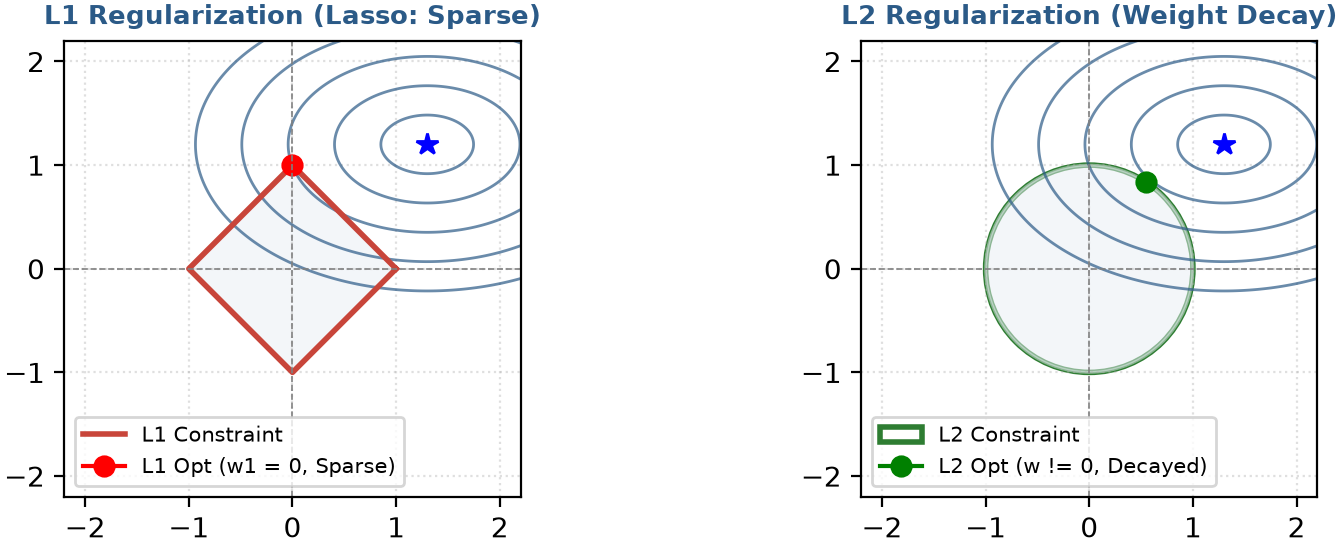
\includegraphics[width=0.58\textwidth]{nn1_l1_l2_geometry.png}\\[-1pt]
{\footnotesize\textit{Geometric intuition: $L_1$ diamond corners touch contours on axes ($w_1 = 0 \implies$ sparsity); $L_2$ circular ball shrinks weights smoothly without setting them strictly to zero.}}
\end{center}

\vspace{-6pt}

% Side-by-Side L1 vs L2 Mathematical Derivation
\noindent\begin{minipage}[t]{0.485\textwidth}
\begin{tcolorbox}[
    colframe=themeblue, colback=lightbg, coltitle=white,
    fonttitle=\bfseries\sffamily\small,
    title={$L_2$ Regularization (Ridge / Weight Decay)},
    arc=1.3mm, boxrule=0.5pt, left=4pt, right=4pt, top=2pt, bottom=2pt
]
\footnotesize
\textbf{Complexity Penalty (Squared $L_2$ Norm):}
\[
\Omega_{L2}(w) = \frac{\lambda}{2m} \|w\|_2^2 = \frac{\lambda}{2m} \sum_{j=1}^{n_x} w_j^2
\]
\textbf{Total Cost Function:}
\[
J(w, b) = \frac{1}{m}\sum_{i=1}^m \mathcal{L}\big(\hat{y}^{(i)}, y^{(i)}\big) + \frac{\lambda}{2m} \|w\|_2^2
\]
\hrulefill\\[1pt]
\textbf{Gradient with Regularization:}
\[
\frac{\partial J}{\partial w} = \frac{\partial J_{\text{orig}}}{\partial w} + \frac{\lambda}{m} w
\]
\textbf{Gradient Descent Update Rule:}
\begin{align*}
w &:= w - \alpha \frac{\partial J}{\partial w} = w - \alpha \left(\frac{\partial J_{\text{orig}}}{\partial w} + \frac{\lambda}{m} w\right) \\[1pt]
&:= w - \alpha \frac{\lambda}{m} w - \alpha \frac{\partial J_{\text{orig}}}{\partial w} \\[2pt]
&:= \underbrace{\left(1 - \alpha \frac{\lambda}{m}\right)}_{< 1} w - \alpha \frac{\partial J_{\text{orig}}}{\partial w}
\end{align*}
\textbf{Key Mathematical Insights:}
\begin{itemize}[leftmargin=7pt, itemsep=0.5pt]
    \item \textbf{Weight Decay:} Pre-multiplication by $\left(1 - \alpha \frac{\lambda}{m}\right) < 1$ shrinks weights at every update.
    \item \textbf{Smooth Shrinkage:} Heavily penalizes large weights; smoothly decays small weights.
\end{itemize}
\end{tcolorbox}
\end{minipage}
\hfill
\begin{minipage}[t]{0.485\textwidth}
\begin{tcolorbox}[
    colframe=accentred, colback=white, coltitle=white,
    fonttitle=\bfseries\sffamily\small,
    title={$L_1$ Regularization (Lasso / Sparsity)},
    arc=1.3mm, boxrule=0.5pt, left=4pt, right=4pt, top=2pt, bottom=2pt
]
\footnotesize
\textbf{Complexity Penalty (Absolute $L_1$ Norm):}
\[
\Omega_{L1}(w) = \frac{\lambda}{m} \|w\|_1 = \frac{\lambda}{m} \sum_{j=1}^{n_x} |w_j|
\]
\textbf{Total Cost Function:}
\[
J(w, b) = \frac{1}{m}\sum_{i=1}^m \mathcal{L}\big(\hat{y}^{(i)}, y^{(i)}\big) + \frac{\lambda}{m} \|w\|_1
\]
\hrulefill\\[1pt]
\textbf{Subgradient with Regularization ($w_j \neq 0$):}
\[
\frac{\partial J}{\partial w} = \frac{\partial J_{\text{orig}}}{\partial w} + \frac{\lambda}{m} \text{sign}(w)
\]
\textbf{Gradient Descent Update Rule:}
\begin{align*}
w &:= w - \alpha \frac{\partial J}{\partial w} = w - \alpha \left(\frac{\partial J_{\text{orig}}}{\partial w} + \frac{\lambda}{m} \text{sign}(w)\right) \\[2pt]
&:= w - \alpha \frac{\partial J_{\text{orig}}}{\partial w} - \underbrace{\alpha \frac{\lambda}{m} \text{sign}(w)}_{\text{constant shift towards } 0}
\end{align*}
\textbf{Key Mathematical Insights:}
\begin{itemize}[leftmargin=7pt, itemsep=0.5pt]
    \item \textbf{Constant Shrinkage:} Shifts weights toward 0 by a fixed amount regardless of magnitude.
    \item \textbf{Sparse Weights:} Drives coefficients \textbf{strictly to zero}, yielding automatic feature selection.
\end{itemize}
\end{tcolorbox}
\end{minipage}

\vspace{1pt}

\begin{tcolorbox}[
    colframe=themeblue, colback=lightbg, arc=1.3mm, boxrule=0.5pt,
    left=5pt, right=5pt, top=2pt, bottom=2pt
]
\footnotesize
\textbf{Intuition: Why Regularization Prevents Overfitting:}
Consider hidden units utilizing activation $g(z) = \tanh(z)$:
\[
\text{Increasing } \lambda \quad\Longrightarrow\quad \text{Shrinks weights } w \approx 0 \quad\Longrightarrow\quad z = w^T x + b \approx 0
\]
When linear logits $z$ are concentrated near $0$, $\tanh(z)$ is restricted to its approximately linear regime ($\tanh(z) \approx z$ with derivative $g'(z) \approx 1$). As proven in Section 2, a network operating under linear activations collapses toward a simple linear model. Hence, strong regularization naturally limits network capacity, preventing complex high-frequency oscillations and eliminating overfitting.
\end{tcolorbox}

\end{document}
